\documentclass[11pt]{beamer}
\usetheme{CambridgeUS}
\usepackage[utf8]{inputenc}
\usepackage[german]{babel}
\usepackage[T1]{fontenc}
\usepackage{amsmath}
\usepackage{amsfonts}
\usepackage{amssymb}
\usepackage{graphicx}
\usepackage{animate,media9,movie15}
\author{Timo Briddigkeit \and Johannes Selymes}
\title{SPV\\QuadGui}
\setbeamercovered{transparent} 
\setbeamertemplate{navigation symbols}{} 
\logo{\includegraphics[width=0.8cm,height=0.6cm]{fhlogo.png} } 
%\institute{FH Hagenberg} 
\date{\today} 
%\subject{} 

%%%%%%% die folgende Sequenz blendet mit jeder neuen Section einmal das 
%%%%%%% Inhaltsverzeichnis mit dem Titel "Übersicht" ein und markiert den
%%%%%%% jeweils aktuellen Gliederungspunkt
\AtBeginSection[]{
\begin{frame}<beamer>
\frametitle{Übersicht} 
\tableofcontents[currentsection,currentsubsection]
\end{frame}
}

\begin{document}

\begin{frame}
\titlepage
\end{frame}

\begin{frame}{Inhalt}
\tableofcontents
\end{frame}

\section{Einleitung}
\section{QuadGui}
\begin{frame}
\begin{figure}
\centering
\includegraphics[scale=0.5]{gui.png} 
\caption{Die WPF-Application}
\end{figure}
\end{frame}
\section{QuadServer}
\begin{frame}
\begin{figure}
\centering
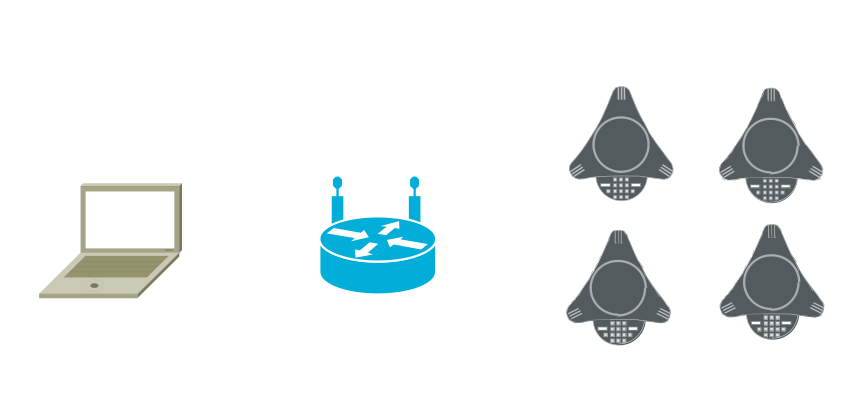
\includegraphics[scale=0.5]{comm.png} 
\caption{Die Netzwerkkommunikation}
\end{figure}
\end{frame}


\end{document}